\documentclass[12pt]{exam}

\usepackage[brazil]{babel}   
\usepackage[TS1,T1]{fontenc}
\usepackage[utf8]{luainputenc}
\usepackage[utf8]{inputenc}  
%\usepackage[T1]{fontenc}
\usepackage{amsfonts,amsmath,amssymb,latexsym} 
\usepackage{enumerate}
\usepackage{float}
\usepackage{graphicx}
\usepackage{caption}
\usepackage{subcaption}
\graphicspath{ {images/} }




\def\cQ{\mathcal{Q}}
\def\ve{\varepsilon}

\def\emptyset{\varnothing}
\def\ept{\varnothing}

% Include the listings-package
\usepackage{listings}             
\usepackage{color}

\definecolor{dkgreen}{rgb}{0,0.6,0}
\definecolor{gray}{rgb}{0.5,0.5,0.5}
\definecolor{mauve}{rgb}{0.58,0,0.82}

\lstset{frame=tb,
  language=Prolog,
  aboveskip=3mm,
  belowskip=3mm,
  showstringspaces=false,
  columns=flexible,
  basicstyle={\small\ttfamily},
  numbers=left,
  stepnumber=1,  
  numberstyle=\tiny\color{gray},
  keywordstyle=\color{blue},
  commentstyle=\color{dkgreen},
  stringstyle=\color{mauve},
  breaklines=true,
  breakatwhitespace=true,
  tabsize=3
}


\usepackage{tikz}
\usetikzlibrary{trees}



\usepackage[margin=1in]{geometry}
\usepackage{amsmath,amssymb}
\usepackage{multicol}

\def\code#1{\texttt{#1}}

\newcommand{\class}{IA}
\newcommand{\term}{1º semestre de 2021}
\newcommand{\examnum}{Lista 04}
\newcommand{\examdate}{}

\pointpoints{ponto}{pontos}

\pagestyle{head}
\firstpageheader{}{}{}
\runningheader{\class}{\examnum\ - Página \thepage\ de \numpages}{\examdate}
\runningheadrule


\begin{document}

\noindent
\begin{tabular*}{\textwidth}{l @{\extracolsep{\fill}} r @{\extracolsep{6pt}} l}
\textbf{\class} & \textbf{Nome:} & \makebox[2in]{\hrulefill}\\
\textbf{\term}  & \textbf{RA:}   & \makebox[2in]{\hrulefill}\\
\textbf{\examnum} &&\\
& Professor: & Vinicius Pereira
\end{tabular*}\\
\rule[2ex]{\textwidth}{2pt}

Esta lista contém \numpages\ páginas e \numquestions\ questões.\\


\noindent
\rule[2ex]{\textwidth}{2pt}


\vspace{3em}




\begin{description}

\item[Procedimento minimax]:\\
Se a árvore é exaustivamente buscável abra todos os vértices e escolha uma avaliação para cada resultado.\\
Se não, abra até certo nível e escolha uma heurística de avaliação para cada vértice resultado.\\
Na implementação, rotulamos cada nível da busca de acordo com quem joga neste ponto do jogo: MIN, ou MAX.\\
Cada vértice folha recebe uma avaliação.\\
O procedimento propaga estes valor para os vértices ancestrais de acordo com a seguinte regra:\\
\begin{description}
  \item Se o estado pai for um vértice MAX dê-lhe o valor máximo entre seus filhos - esta é a escolha do jogador que quer maximizar o ganho.\\
  \item Se o estado pai for um vértice MIN dê-lhe o valor mínimo entre seus filhos - esta é a escolha do jogador que quer minimizar o ganho do jogador MAX.\\
\end{description}

\break




\item[Poda Alfa-Beta]
O procedimento inicial é fazer uma busca em profundidade para termos um valor inicial, com este valor criamos valores $\alpha$ e $\beta$ para os vértices ancestrais da folha encontrada.
\begin{description}
  \item Associa um valor $\alpha$ para cada vértice de MAX, este valor representa o melhor (mais alto) valor que foi encontrado até agora nos caminhos de uma folha para este vértice.
  \item Associa um valor $\beta$ para cada vértice de MIN, este valor representa o melhor (mais baixo) valor que foi encontrado até agora nos caminhos de uma folha para este vértice.
\end{description}
A seguinte regra é aplicada:
\begin{description}
  \item A poda pode ser feita abaixo de qualquer vértice MIN que tenha um valor $\beta$ menor, ou igual, que o valor $\alpha$ de qualquer um dos seus ancestrais MAX.
  \item A poda pode ser feita abaixo de qualquer vértice MAX que tenha um valor $\alpha$ maior, ou igual, que o valor $\beta$ de qualquer um dos seus ancestrais MIN.
\end{description}
Note que valores $\alpha$ não diminuem e valores $\beta$ não aumentam.



\end{description}

\vspace{3em}

\begin{questions}

\question Considere a árvore da figura \ref{fig:treeGameMinMax01}, propague os valores das folhas até a raíz, usando o procedimento Minimax.

Faça a poda alfabeta da esquerda para a direita e da direita para a esquerda.

\begin{figure}[h]
    \centering
    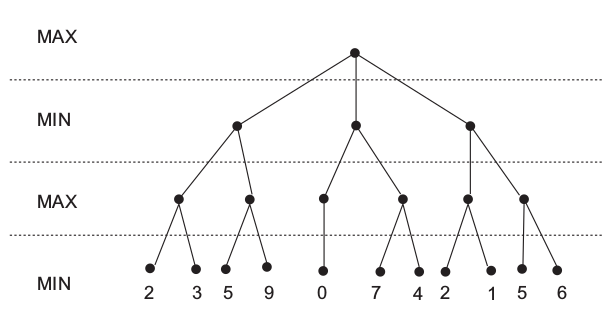
\includegraphics[width=0.60\textwidth]{treeGameMinMax01}
    \caption{Uma árvore para o procedimento Minimax.}
    \label{fig:treeGameMinMax01}
\end{figure}




\break


\question Considere a árvore da figura \ref{fig:treeGameMinMax02}, propague os valores das folhas até a raíz, usando o procedimento Minimax.

Faça a poda alfabeta da esquerda para a direita e da direita para a esquerda.

\begin{figure}[h]
    \centering
    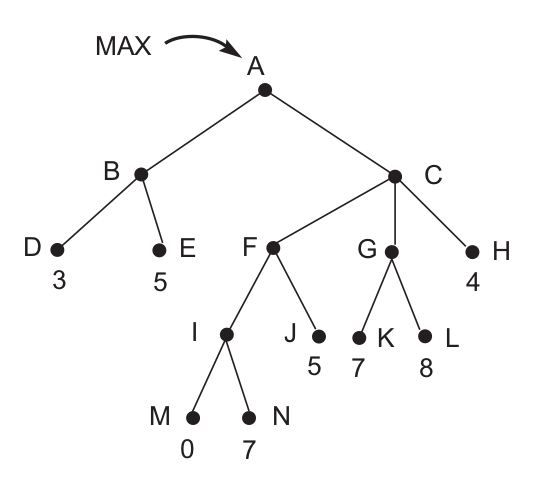
\includegraphics[width=0.60\textwidth]{treeGameMinMax02}
    \caption{Uma árvore para o procedimento Minimax.}
    \label{fig:treeGameMinMax02}
\end{figure}





\question Considere uma variante do jogo \textit{nim}, diversas fichas são colocadas sobre a mesa formando pilhas, em cada rodada um dos jogadores deve dividir uma das pilhas em duas pilhas sem que as duas pilhas resultantes tenham quantidade de fichas iguais. O jogador que não conseguir fazer uma jogada perde o jogo.

Para o jogo com dois jogadores, com o jogador MAX começando, faça uma busca exaustiva (até o último nível) para um estado inicial de uma pilha com 8 fichas, e para um estado inicial de uma pilha com 9 fichas. Observe estados semelhantes.

Atribua um valor para cada folha e faça a propagação dos valores das folhas nas duas árvores, evidenciando a jogada de cada jogador.



\question Considere o seguinte jogo ``simples'' para duas pessoas. Em um tabuleiro com $n$ casas alinhadas, enumeradas de $1$ a $n$, sendo a casa $i$ vizinha à casa $i+1$ e $i-1$ e a mais nenhuma outra, a casa $1$ vizinha à casa $2$ e a casa $n$ vizinha à casa $n-1$ e a mais nenhuma outra. 
Cada jogador tem apenas uma peça que pode ocupar uma casa. 
Em cada turno um jogador deve mover a sua peça e este movimento pode ser para uma casa vizinha, caso esta esteja vaga; ou pular a peça do adversário movendo-se para a casa vizinha à peça do adversário, caso a peça do adversário esteja em uma casa vizinha. A peça do jogador $A$ começa na casa $1$ e a peça do jogador $B$ começa na casa $n$. O objetivo de cada jogador é chegar com a sua peça na casa outra extremidade, quem chegar primeiro ganha.

Um exemplo deste jogo com $4$ casas pode ser visto na figura \ref{fig:simpleGame4}.

Abra uma árvore de estados para o jogo com $4$ e com $5$ casas. Reprente cada estado como $(S_A, S_B)$, onde $S_X$ é o número da casa do jogador $X$. Caso algum caminho entre em loop, junte os dois vértices repetidos e coloque seu valor como `$?$'.

Qual jogador ganhará em cada caso?

\begin{figure}[h]
    \centering
    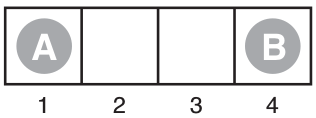
\includegraphics[width=0.40\textwidth]{simpleGame4}
    \caption{O jogo ``simples'' com $4$ casas.}
    \label{fig:simpleGame4}
\end{figure}



\question Considere a heurística da figura \ref{fig:tictacHeu} para o jogo da velha. 

As árvores das figuras \ref{fig:tictacPoda01}, \ref{fig:tictacPoda02} e \ref{fig:tictacPoda03} são execuções do algoritmo Minimax com dois níveis de profundidade.

Redesenhe estas árvores aplicando a poda alfabeta, sendo que você pode escolher a ordem dos caminhos a percorrer.

\begin{figure}[h]
    \centering
    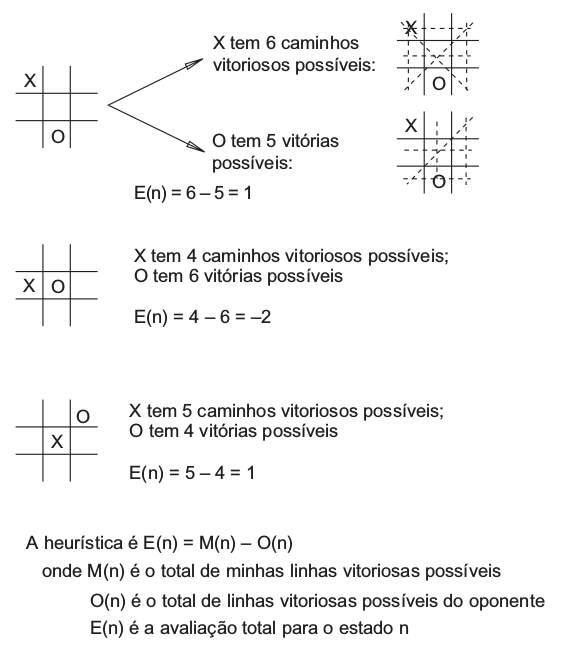
\includegraphics[width=0.90\textwidth]{tictacHeu}
    \caption{Heurística para o jogo da velha.}
    \label{fig:tictacHeu}
\end{figure}

\begin{figure}[h]
    \centering
    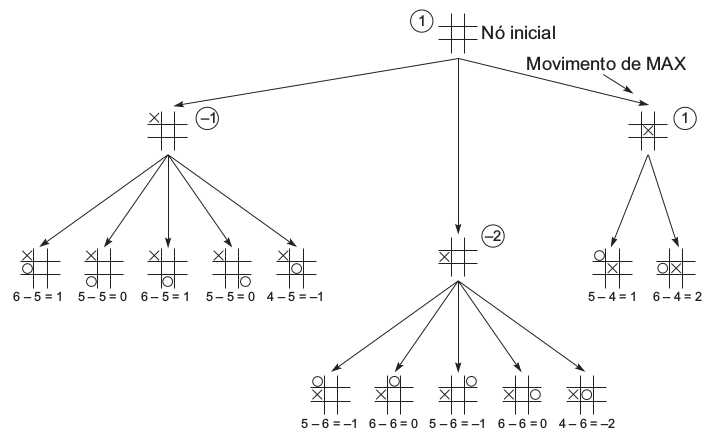
\includegraphics[width=0.90\textwidth]{tictacPoda01}
    \caption{Iteração 1 para o procedimento Minimax com dois níveis.}
    \label{fig:tictacPoda01}
\end{figure}

\begin{figure}[h]
    \centering
    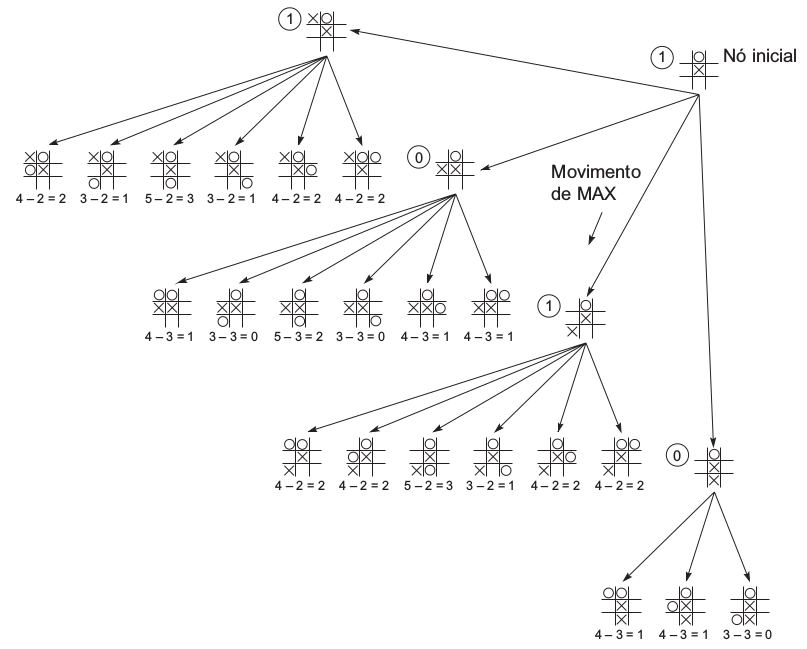
\includegraphics[width=0.90\textwidth]{tictacPoda02}
    \caption{Iteração 2 para o procedimento Minimax com dois níveis.}
    \label{fig:tictacPoda02}
\end{figure}

\begin{figure}[h]
    \centering
    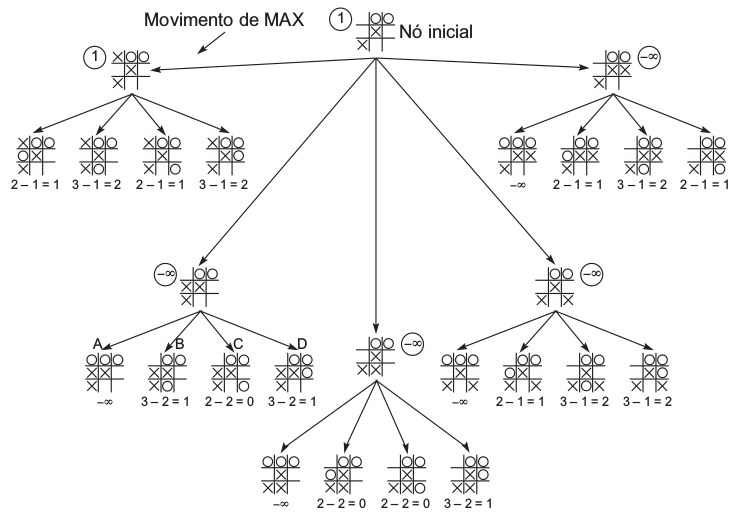
\includegraphics[width=0.90\textwidth]{tictacPoda03}
    \caption{Iteração 3 para o procedimento Minimax com dois níveis.}
    \label{fig:tictacPoda03}
\end{figure}

\end{questions}



\end{document}

